\documentclass[twosided]{article}
\setlength{\oddsidemargin}{0.25 in}
\setlength{\evensidemargin}{-0.25 in}
\setlength{\topmargin}{-0.6 in}
\setlength{\textwidth}{6.5 in}
\setlength{\textheight}{8.5 in}
\setlength{\headsep}{0.75 in}
\setlength{\parindent}{0 in}
\setlength{\parskip}{0.1 in}

\usepackage{amsmath,amsfonts,graphicx,algorithm,caption}
\usepackage{cite}
\usepackage[document]{ragged2e}
\usepackage{graphicx}
\usepackage{subfigure}
\usepackage[english]{babel}
\usepackage{url}

\newcommand{\lecture}[3]{
   \pagestyle{myheadings}
   \thispagestyle{plain}
   \newpage
   \noindent
   \begin{center}
   \framebox{
      \vbox{\vspace{2mm}
    \hbox to 6.28in { {\bf IE643: Deep Learning : Theory and Practice
		\hfill Aug-Dec 2020} }
       \vspace{4mm}
       \hbox to 6.28in { {\Large \hfill Quiz #1  \hfill} }
       \vspace{2mm}
       \hbox to 6.28in { {\it Lecturer: #2 \hfill #3} }
      \vspace{2mm}}
   }
   \end{center}
}

\begin{document}
\lecture{3}{P. Balamurugan}{Shashank Kumar (170050031)}

\section{Question 1}

\subsection{Part (a)}
Deep convolutional networks like VGGNet, ResNet which are trained on datasets like Pascal VOC and Imagenet cannot be used to perform the object detection tasks. Environmental conditions like mist, pollution, smoke and dust lead to poor quality images. The objects in the images are not clearly visible due to smoke and mist. Such conditions hinder the visibility level in an image and therefore, bounding boxes are either not generated around the less visible objects or the box isn't accurate and the object is not recognizable in the image. Many state-of-the-art object detection algorithms have failed to generate the desired output with such images. 
    \begin{figure}[h]
        \centering
        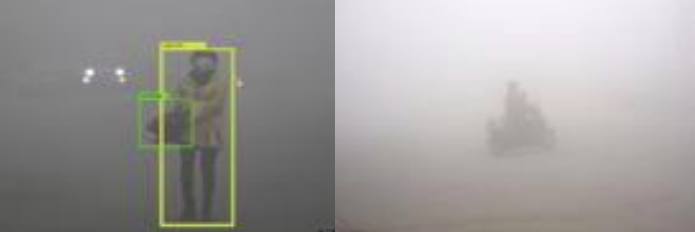
\includegraphics[width=0.7\textwidth]{images/Figure1.png}
        \caption{Faster R-CNN fails to detect objects}
        \label{fig:figure1}
    \end{figure}

\subsection{Part (b)}
The architecture that would help with the task at hand can use a combination of image enhancement neural network followed by classical object detection and recognition networks.
\begin{enumerate}
    \item \textbf{Image enhancement:} \\
    Deep neural networks for image enhancement have been proposed like \cite{DeepPhoto} and \cite{EnhanceImage}. The network in \cite{EnhanceImage} accepts a foggy image and renders an enhanced version. The datasets to be used are described in part (c). The output image generated by this network is compared with the ground truth images. Squared-error loss function is used in this case. The results can be seen in figure \ref{fig:figure2}.
    \item \textbf{Object recognition and detection:} \\
    The enhanced images obtained can be used for object detection tasks with the deep convolutional networks like Faster-RCNN and YOLO. A few other research paper like \cite{Salient} use saliency map for better estimation of bounding boxes. Saliency map is a topographical representation of the visually alluring locations in an image. The saliency map of the images under foggy conditions have distinct and clear boundaries.  
\end{enumerate}

\begin{figure}[h]
    \centering
    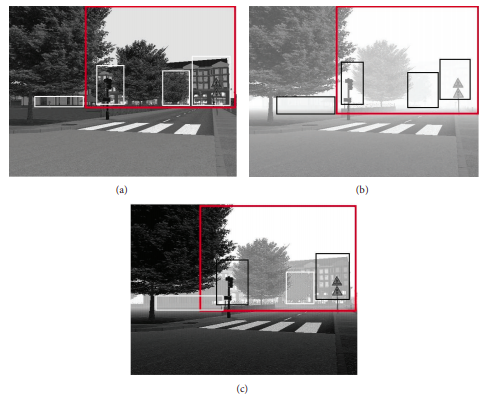
\includegraphics[width=0.7\textwidth]{images/Figure2.png}
    \caption{(a) Original scene without fog. (b) Scene visibility degraded under fog. (c) Visibility enhancement by deep neural network.}
    \label{fig:figure2}
\end{figure}  

\textbf{Proposed neural network architecture:}\\
The figure \ref{fig:figure3} shows the neural network architecture proposed in \cite{Salient}. Instead of using Faster-RCNN, YOLO architecture can be used for faster real-time performance. The loss function consists of a penalty term for bad localization of the center of the bounding box, a penalty for wrong height and width estimation of the bounding box and squared loss for the confidence scores

\begin{figure}[h]
    \centering
    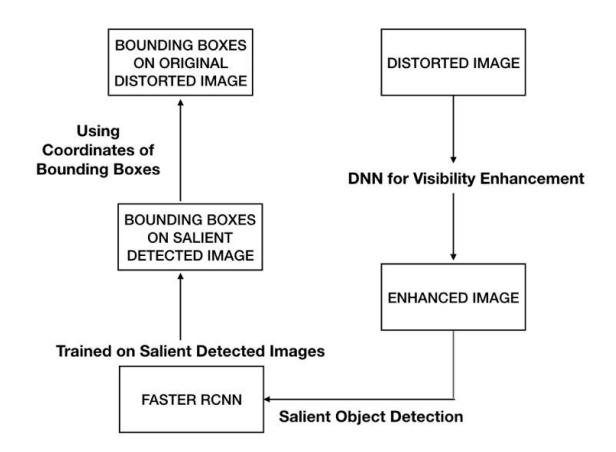
\includegraphics[width=0.7\textwidth]{images/Figure3.png}
    \caption{Neural network with image enhancement and object detection}
    \label{fig:figure3}
\end{figure}

\subsection{Part (c)}
FRIDA (Foggy Road Image DAtabase) image database comprises of 90 synthetic images of 18 urban road scenes. FRIDA2 comprises 330 synthetic images of 66 diverse road scenes. SHIA (Spectral Hazy Image database for Assessment) is composed of 1540 images with 10 levels of fog each and their corresponding fog-free (ground-truth) images. Pascal VOC dataset can be used after preprocessing the images. A blur can be applied to each of the image while maintaining the same bounding box. The blur intensity is subjective to the image. Image enhacement neural network can use all the three datasets along with the ground truth images. The object detection neural network can be trained on the modified Pascal VOC dataset with blur. 

\section{Question 2}

\subsection{Part (a)}
YOLO (You Only Look Once) algorithm \cite{YOLO} can be used for the detection of animated characters in the frames. Since we are considering real-time detection i.e. capturing frames from the video, YOLO is the obvious choice owing to the high detection speed. The architecture is depicted in the figure \ref{fig:figure4}. \\

\begin{figure}[h]
    \centering
    \includegraphics[width=0.8\textwidth]{images/Figure4.png}
    \caption{YOLO Architecture}
    \label{fig:figure4}
\end{figure}

\newpage

\textbf{Architecture:} \\
In our case, the output of the algorithm are the probability that there is an animated character in the frame, the coordinates of the center, and the height and width of the bounding box relative to the image size. There is just one class label since we only want to detect the animated objects and not classify them. The algorithm segments the image into cells and each cell is assigned the class probability. A maximum over the class probabilities is then assigned to each cell. The image then looks as shown in figure \ref{fig:figure5}. The next step involves non-max suppression which involves combining overlapping bounding boxes using intersection-over-union method. This step is depicted in figure \ref{fig:figure6} which results in the final bounding box. \\

\begin{figure}[h]
    \centering
    \includegraphics[width=0.7\textwidth]{images/Figure5.png}
    \caption{Image divided into cells with class probabilities}
    \label{fig:figure5}
\end{figure}

\begin{figure}[h]
    \centering
    \includegraphics[width=0.7\textwidth]{images/Figure6.png}
    \caption{Non-max suppression}
    \label{fig:figure6}
\end{figure}

\textbf{Loss function:} \\
The loss function used in YOLO algorithm comprises of the sum of the following three components:
\begin{enumerate}
    \item \textbf{a classification loss} over all the cells with the conditional class probabilities given by 
    \[ \sum_{i=0}^{S^2} 1_i^{obj} \sum_{c \in C} (p_i(c) - \hat{p_i}(c))^2 \]
    where \\
    \( 1_i^{obj} = 1\) if the object is in $i$-th cell, otherwise 0 \\
    \( \hat{p_i}(c) \) denotes the conditional probability that a class $c$ appears in the $i$-th cell
    \item \textbf{a localization loss} corresponding to the bounding box which is as follows
    \[ \lambda_{coord} \left( \sum_{i=0}^{S^2} \sum_{j=0}^{B} 1_{ij}^{obj} \left[(x_i - \hat{x_i})^2 + (y_i - \hat{y_i})^2 + (\sqrt{w_i} - \sqrt{\hat{w_i}})^2 + (\sqrt{h_i} - \sqrt{\hat{h_i}})^2 \right] \right) \]
    where \\ 
    \( 1_{ij}^{obj} = 1\) if the $j$-th boundary box in the $i$-th cell is responsible for detecting the object, otherwise 0 \\
    $\lambda_{coord}$ increases the weight for the loss in the boundary box coordinates
    \item \textbf{a confidence loss} based on whether the object is present or not given as
    \[ \sum_{i=0}^{S^2} \sum_{j=0}^{B} \left[ 1_{ij}^{obj} (C_i - \hat{C_i})^2 + \lambda_{noobj} 1_{ij}^{noobj} (C_i - \hat{C_i})^2 \right] \]
    where \\
    \( 1_{ij}^{noobj} \) is the complement of \( 1_{ij}^{obj}\) \\
    \( C_i \) is the box confidence score of box $j$ in cell $i$ \\
    $\lambda_{noobj}$ scales down the loss when detecting background
\end{enumerate}

\textbf{Capturing frames:} \\
To capture the frames with animated character(s), record the frames with atleast one bounding box. Script can be written to take video as input and returning all such frames.

\subsection{Part (b)}
No publically available datasets for the purpose were found.

\subsection{Part (c)}
Datasets can be generated using overlapping cartoon characters on image datasets like Pascal VOC. The data, however, needs to be in a predefined format as per YOLO. The center of the animated character image along with the height and width need to scaled with the image dimensions that it is being overlapped with. There can be multiple characters in an image. The class of all the animated characters can be set to 1. This augmented dataset can be mixed with the original one to generate final dataset.

\subsection{Part (d)}
The dataset generated above can be mixed before splitting it into 3 sets (considering the dataset size of approximately 40000) -
\begin{itemize}
    \item \textbf{a training set} to train the neural network, consisting of approximately 80 percent of data
    \item \textbf{a dev set} to test the trained model and tune the model based on the observations, approximately 10 percent of data
    \item \textbf{a test set} to test the finally ready deployable mode, with the rest 10  percent of data 
\end{itemize}
The trained model can be run on the movie and it would produce bounding boxes for the frames with the animated characters.

\subsection{Part (e)}
The above proposed network already generates the bounding boxes around the animated characters in the frame. No change is required with respect to the datasets, the network architecture and the training procedure.

\begin{thebibliography}{99}
\bibitem{DeepPhoto}
\textit{Deep Photo: Model-Based Photograph Enhancement and Viewing}
Johannes Kopf, Boris Neubert, Billy Chen, Michael F. Cohen, Daniel Cohen-Or, Oliver Deussen, Matt Uyttendaele, Dani Lischinski
\bibitem{EnhanceImage}
\textit{Visibility Enhancement of Scene Images Degraded by Foggy Weather Conditions with Deep Neural Networks}
Farhan Hussain and Jechang Jeong
\bibitem{Salient}
\textit{Intelligent Detection in Less Visibility by Saliency Techniques and Faster Region-based Convolutional Neural Networks}
Sanjay Kumar, Dipti Lohia, Darsh Pratap and Ashutosh Krishna
\bibitem{YOLO}
\textit{You Only Look Once: Unified, Real-Time Object Detection}
Joseph Redmon, Santosh Divvala, Ross Girshick and Ali
\end{thebibliography}

\end{document}
